 % mainfile: ../../../../master.tex
\subsection{Migrate Zicheng's code}
\label{task:20240305_aosp}

\subsubsection{Code differencing}

\begin{longtable}{p{.15\linewidth}p{.40\linewidth}p{.40\linewidth}} 
\toprule
file & 13 to Debloated 13 & 13 to 14 \\
\midrule
\endhead

\path{art_dex_file_loader.cc}
& No change
& Removed MemMapContainer. Replace \texttt{DexFileLoader::OpenCommon} now protected with \texttt{ArtDexFileLoader::Open}, and remove its other overloads.
\\

\path{dex_file_loader.cc}
& No change
& Remove \texttt{DexFileLoader::GetMultiDexChecksums}, \texttt{DexFileLoader::OpenAll}, \texttt{DexFileLoader::OpenOneDexFileFromZip}, \texttt{DexFileLoader::OpenAllDexFilesFromZip}. Modified \texttt{DexFileLoader::Open} and added its overloads, \texttt{DexFileLoader::OpenCommon} and added its overloads. Added \texttt{DexFileLoader::InitAndReadMagic}, \texttt{DexFileLoader::OpenWithDataSection}, \texttt{DexFileLoader::OpenFromZipEntry}
\\

\path{native_loader.cpp}
& Trivial loggings
& No change
\\

\path{native_loader_namespace.cpp}
& Trivial loggings
& No change
\\

\path{odrefresh.cc}
& Change from \path{args.emplace_back("--compiler-filter=speed");} to \path{args.emplace_back("--compiler-filter=verify");}
& Tons of change
\\

\path{quick_trampoline_entrypoints.cc}
& No change
& Lots of change
\\

\path{interpreter_common.cc}
& Trivial Logging
& Modified \path{ShouldStayInSwitchInterpreter}, \path{MoveToExceptionHandler}, \path{DoCallCommon}, \path{ArtInterpreterToCompiledCodeBridge}, \path{InvokeBootstrapMethod}, \path{DoCall}. Added \path{UnlockHeldMonitors}
\\

\path{interpreter_switch.cc}
& Trivial JNI headers imported
& Modified \path{ShouldStayInSwitchInterpreter}, \path{MoveToExceptionHandler}, \path{DoCallCommon}, \path{ArtInterpreterToCompiledCodeBridge}, \path{InvokeBootstrapMethod}, \path{DoCall}. Added \path{UnlockHeldMonitors}
\\

\path{interpreter_switch_impl-inl.h}
& Trivial JNI headers imported
& Modified template settings for \path{CheckTransactionAbort}, \path{CheckForceReturn}, \path{HandlePendingException}, \path{HandleReturn}, \path{HandleGet}, \path{HandlePut}, \path{HandleInvoke}, \path{RETURN_OBJECT}, \path{MONITOR_ENTER}, \path{MONITOR_EXIT}, \path{NEW_ARRAY}, \path{FILLED_NEW_ARRAY}, \path{FILLED_NEW_ARRAY_RANGE}, \path{ExecuteSwitchImplCpp}. Modified \path{Preamble}, \path{CONST_CLASS}, \path{CHECK_CAST}, \path{INSTANCE_OF}, \path{NEW_INSTANCE}, \path{THROW}, \path{CHECK_CAST}. Added \path{DoAssignabilityChecks}
\\

\path{interpreter_switch_impl.h}
& Trivial logging headers imported
& Modified template settings for \path{ExecuteSwitchImplCpp}, \path{ExecuteSwitchImpl}.
\\

\path{interpreter.cc}
& No changes
& Modified \path{ExecuteSwitch}, \path{Execute}, \path{EnterInterpreterFromInvoke}, \path{EnterInterpreterFromDeoptimize}, \path{EnterInterpreterFromEntryPoint}.
\\

\path{jit.cc}, \path{jit_code_cache.cc}
& No changes
& Changes
\\

\path{java_vm_ext.cc}
& Modified \path{FindSymbol} to check if MINIMA symbol
& Modified \texttt{JavaVMExt::JavaVMExt},  \texttt{JavaVMExt::Create},  \texttt{JavaVMExt::AddGlobalRef},  \texttt{JavaVMExt::AddWeakGlobalRef}, \texttt{JavaVMExt::DeleteGlobalRef}, \texttt{JavaVMExt::DeleteWeakGlobalRef}, \texttt{JavaVMExt::DisallowNewWeakGlobals}, \texttt{JavaVMExt::AllowNewWeakGlobals}, \texttt{JavaVMExt::DecodeGlobal}, \texttt{JavaVMExt::GetIndirectRefKind}, \texttt{JavaVMExt::DecodeWeakGlobalDuringShutdown}, \texttt{JavaVMExt::LoadNativeLibrary}, \texttt{JavaVMExt::FindCodeForNativeMethod}, \texttt{JavaVMExt::GetLibrarySearchPath}. Added \texttt{JavaVMExt::Initialize}, \texttt{JavaVMExt::DecodeWeakGlobalAsStrong}. Remove \texttt{JavaVMExt::SweepJniWeakGlobals}
\\


\midrule
\caption{Differences} 
\label{tab:aospdiff}
\end{longtable}


% 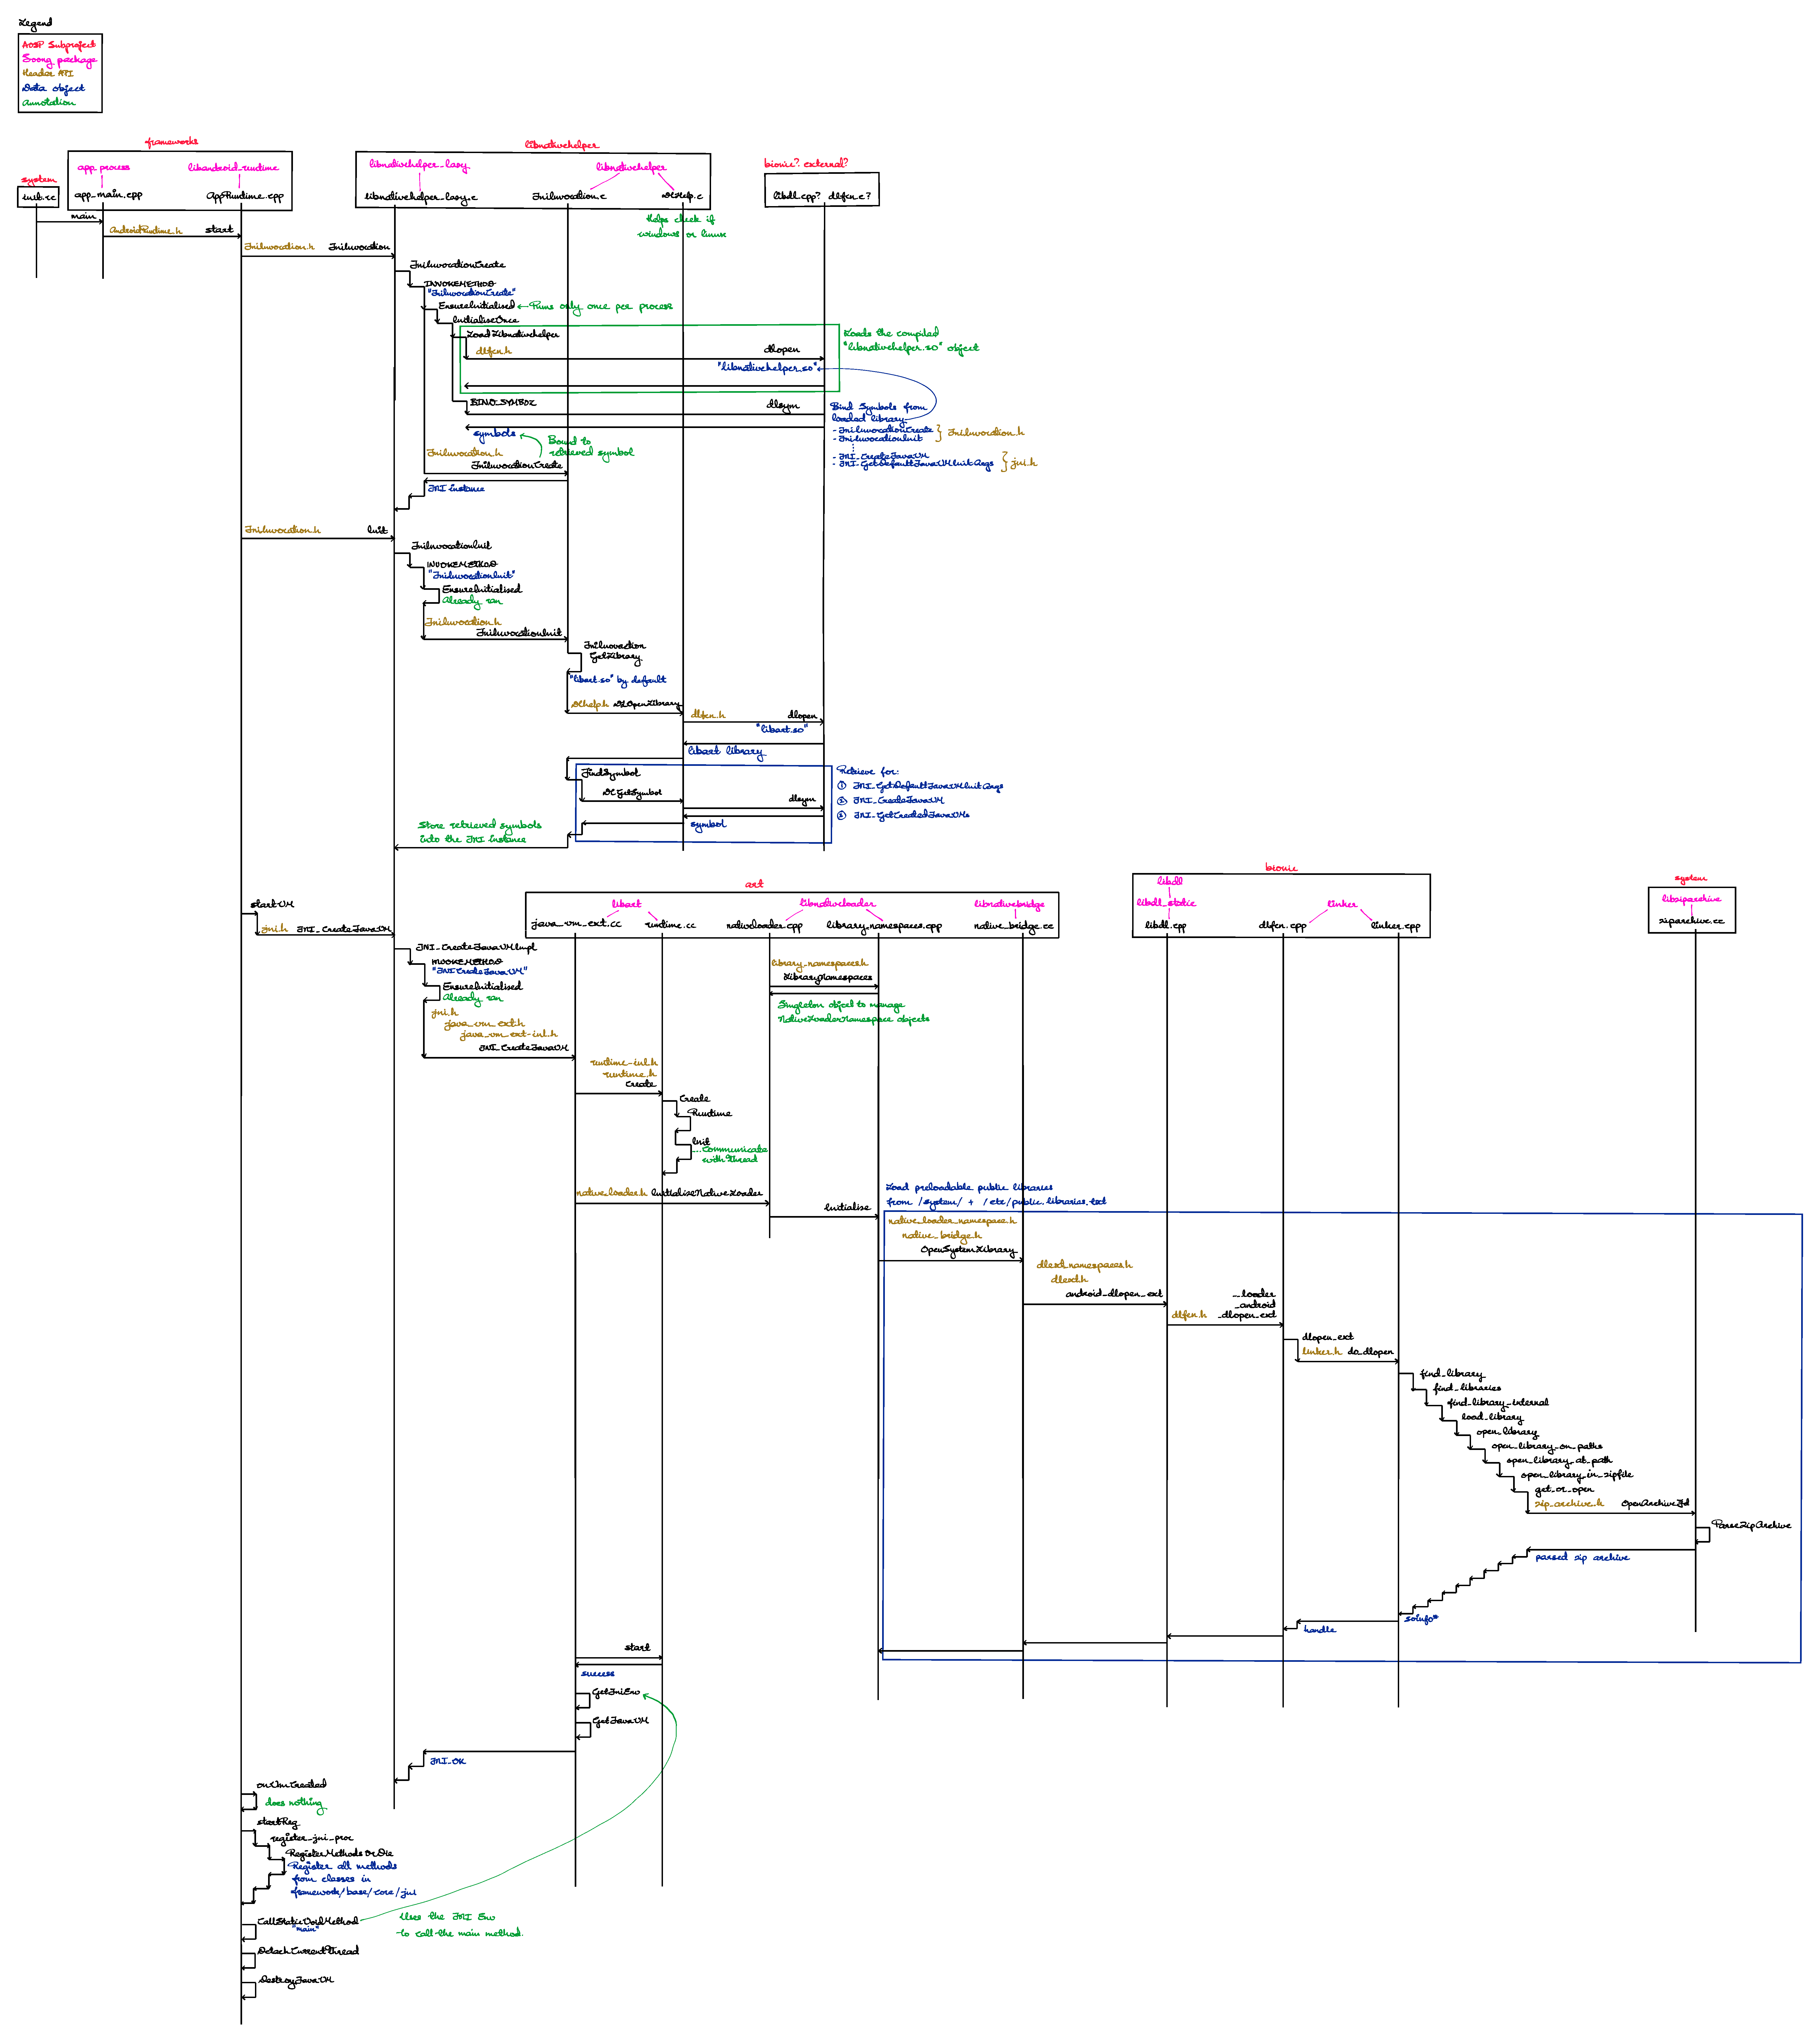
\includepdf[pages=-, scale=.95,pagecommand={}]{entries/2024/01/01/art.pdf}

% \begin{itemize}
% \item \textbf{Domain.} The context of the process that is acting upon something.
% \item \textbf{Type.} The context of the resource on which the process is acting.
% \item \textbf{Class.} The object class of the resource (e.g. \textit{file} or \textit{socket}).
% \item \textbf{Permissions.} The permissions that are allowed given the \textit{domain}, \textit{type} and \textit{class}.
% \end{itemize}

% SELinux rule syntax:
% \begin{lstlisting}
% allow <domain> <type>:<class> { <permissions> };
% \end{lstlisting}

% \subsubsection{Decoding Permission Denial Message}

% Message:
% \begin{lstlisting}
% type=AVC msg=audit(1363289005.532:184): avc:  denied  { read } for  pid=29199 comm="Trace" 
% name="online" dev="sysfs" ino=30 scontext=staff_u:staff_r:googletalk_plugin_t 
% tcontext=system_u:object_r:sysfs_t tclass=file
% \end{lstlisting}

% \begin{longtable}{p{.15\linewidth}p{.15\linewidth}p{.65\linewidth}} 
% \toprule
% Log part & Name & Description \\
% \midrule
% \endhead

% \texttt{type=AVC}
% &Log type
% &Only in the \texttt{audit.log} file; it informs the user what kind of audit log type this is. 
% \\

% \texttt{msg=audit(1363289005.532:184)}
% &Timestamp
% &Timestamp in seconds since epoch, meaning the number of seconds since January 1st, 1970. You can convert this to a more human readable format using date -d @ followed by the number, like so: \texttt{date -d @1363292159.532}.
% \\

% \texttt{avc:}
% &Log type (again)
% &
% \\

% \texttt{ino=30}
% &inode number
% &The inode number of the target file. In this case, since we know it is on the \texttt{sysfs} file system, we can look for this file using: \texttt{find /sys -xdev -inum 30}
% \\

% \texttt{scontent=staff\_u:staff\_r:googletalk\_plugin\_t}
% &Source context
% &The security context of the process (the domain)
% \\

% \texttt{tcontext=system\_u:object\_r:sysfs\_t}
% &Target context
% &The security context of the target resource (in this case the file)
% \\

% \texttt{tclass=file}
% &Target class
% &The class of the target.
% \\

% \midrule
% \caption{Permission Denied Syntax} 
% \label{tab:permissiondeniedsyntax}
% \end{longtable}


% \subsubsection{SELinux Architecture}

% SELinux consists of four main components: object managers (OM), access vector cache (AVC), security server, and security policy as show below:
% \begin{figure}[H]
%     \centering
%     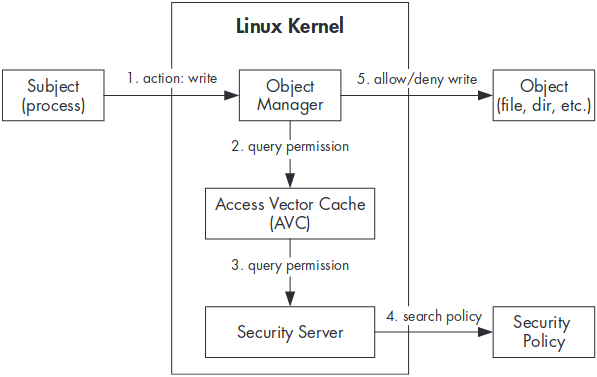
\includegraphics[width=.85\linewidth]{entries/2023/12/10/selinux.png}
%     \caption{SELinux Components}
%     \label{fig:selinux}
% \end{figure}
